\chapter{Web Services for The Internet of Things}
\label{chapter:webservicesfortheiot} 
A Web Service ``is a network accessible interface to application functionality, built using standard Internet technologies'' \cite{snell2009programming}. In other words, an application can be accessed by another application, client or user over the Internet, via web technology such as HTTP, XML or SMTP. A Web Service, usually, provides services based on standards at the layer between service requesters and service providers. This means, it does not matter how are the services implemented, e.g. using C/C++, Java, Python or Javascript, or based on whatever platforms, e.g. Windows Server, Max OS Server or Unix Server. 

When a request is sent to a web service layer, this layer will start a procedure which further requests the service provider. When the procedure is finished, the web service layer will response to the sender results (the response is sometimes optional and it relies on how is the web service implemented). The communication, between the service requesters and the web service layer, is usually based on standard protocols, which aims at cross-platform interoperability. 

The next, we will talk about a sequence of protocols that can be used in Web Services.

\section{REST}
Representational State Transfer (REST) is introduced by ROY T. FIELDING in his doctoral dissertation in 2000. REST is a web architectural style. It is, however, not a standard or protocol. 

An architectural style is ``a coordinated set of architectural constraints that restricts the roles and features of architectural elements, and the allowed relationships among those elements, within any architecture that conforms to the style. Thus, a style provides a name by which we can refer to a packaged set of architectural design decisions and the set of architectural properties that are induced by applying the style.'' \cite {fielding2002principled}

REST was developed in parallel with HTTP protocols with the basic four constraints: resources identified by URI; resources manipulated by standard HTTP methods; resources with various representations; and stateless communication. Resources are data that can be addressed by URIs, which further implies resources are differed by URIs. A representation is a way to present resources. For example, a text, an Image or an HTML document. The representation, moreover, consists of metadata describing the data and, occasionally, metadata describing metadata.

All REST communications are stateless. Thus, each request involves all the necessary information that a receiver needs to understand the request. An example of stateless design is shown in Figure \ref{fig:stateless-design} \cite{rodriguez2008restful}

\begin{figure}[ht]
  \begin{center}
    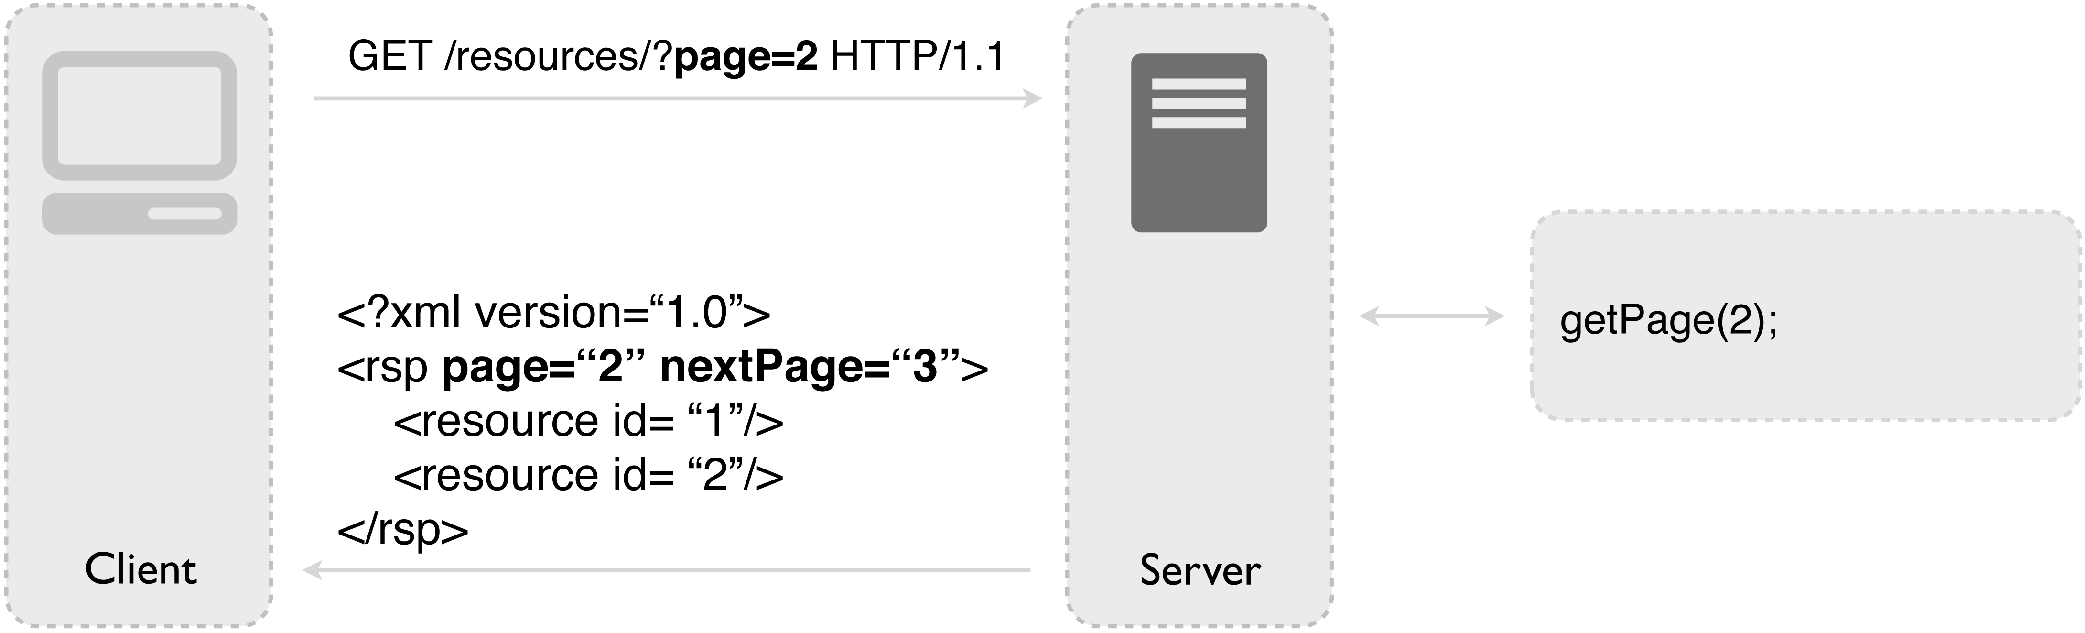
\includegraphics[width=1\textwidth]{images/stateless-design.pdf}
    \caption{Stateless Design}
    \label{fig:stateless-design}
  \end{center}
\end{figure}

As it is illustrated, the request specifies which page the client fetches, i.e. page 2; while the response message contains what the current page is, what the next page is and also the requested page.

On the contrary, stateful design, as shown by Figure \ref{fig:stateful-design} \cite{rodriguez2008restful}, the server saves each client status and responses the corresponding status to the clients who request them. In \ref{fig:stateful-design}, the client need not to specify which page it fetches, but just call the corresponding procedure. The server computes the result and returns the page to the client.

\begin{figure}[ht]
  \begin{center}
    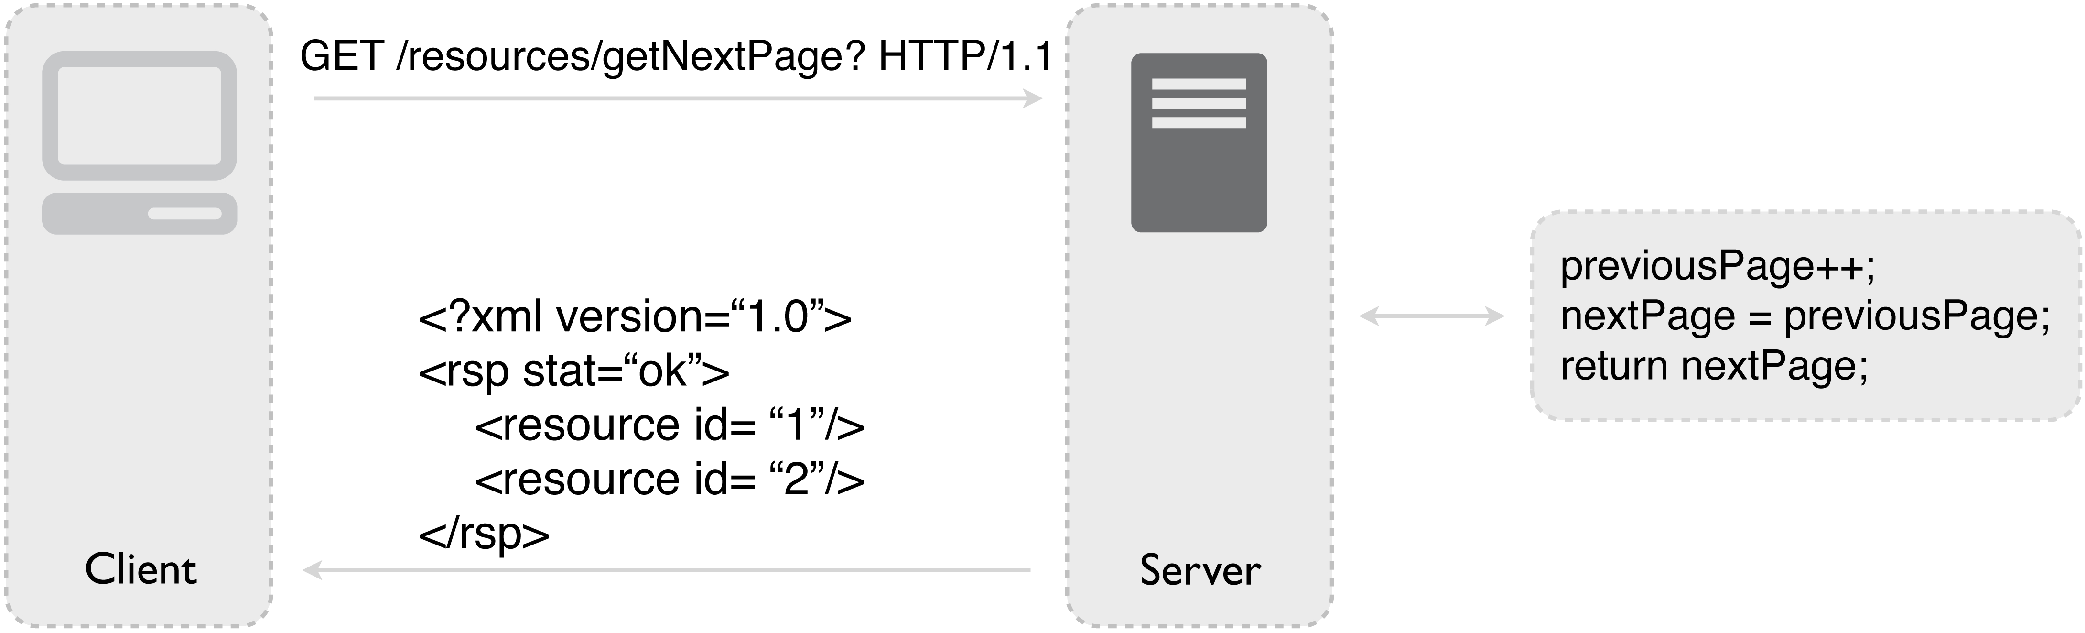
\includegraphics[width=1\textwidth]{images/stateful-design.pdf}
    \caption{Stateful Design}
    \label{fig:stateful-design}
  \end{center}
\end{figure}

The replies are in XML format in Figure \ref{fig:stateless-design} and \ref{fig:stateful-design}, but the REST reply is not restricted in XML document. It could be JSON or other data structure. Usually, REST is implemented relying on HTTP and other web technologies. 

\section{SOAP}
SOAP, a protocol designed for web services, specifies, firstly, a XML-based envelope to transfer information; Secondly, a set of rules for translating application and platform-specific data types into XML representations \cite{snell2009programming}. 

SOAP is largely based on XML standards and provides a standard way to structure XML messages. Thus, SOAP has two related applications: Remote Procedure Call (RPC) and Electronic Document Interchange (EDI). RPC is one way to do distributed computing, where one programme calls a function or method (called procedure) on another, optionally with parameters and receiving return value. EDI is used in automated transactions.

A SOAP message contains an optional SOAP header and a required SOAP body. The SOAP header consists of several information blocks and each of the block is a header. Each header explains how the message is to be parsed. The message body is the actual message in XML syntax. 

SOAP provides a mechanism to handle errors which is called SOAP Faults. A SOAP fault consists of fault code, fault string, the fault actor and the fault details. The fault code has been standardised in namespace belong to \url{http://www.w3.org/2001/06/soap-envelope}; The fault string is an explanation of the error for human to read, while the fault detail is a further explanation about the error. The actor is a concept in SOAP Message Exchange Patterns (MEP), a pattern of message exchanged between SOAP nodes, which has been standardised at \cite{booth2007web}.

When a SOAP message is sent from a provider to a receiver, it passes one or more web services. Each of the web service is called intermediary. All these intermediaries that the SOAP message travels through is called a message path. We call each intermediary on a message path an actor. Thus, the fault actor is the unique identifier of message processing node where the error occurs. 

SOAP does not specify the means of SOAP message transports. Generally, SOAP can be transferred through HTTP, FTP, BSD sockets and SMTP etc. 

\section{CoAP}
Constrained RESTful Environments (CORE) is a working group under Internet Engineering Task Force (IETF) foaming in 2010\footnote{https://datatracker.ietf.org/wg/core/history/}. CORE has been contributing the major standardisation work for Constrained Application Protocol (CoAP). 

CoAP is a protocol (in draft) used in constrained nodes and constrained networks and designed for machine-to-machine (M2M) applications \cite{shelby2013constrained}. A constrained node, usually, has a lower capacity controller with a small amount of ROM and RAM. Constrained networks refer to the networks, generally, with high packets error rates and a low throughput.

CoAP applications or endpoints interact via a request/response model. It also supports built-in services and resources discoveries. With CoAP, applications or endpoints can easily interact with an HTTP based web architecture. \cite{shelby2013constrained} 

Unlike HTTP, CoAP stack is designed for constrained environment, while CoAP, additionally, differ from HTTP in terms of power consumption and overhead. Generally, CoAP power consumption bytes per-transaction are lower than those of HTTP, which implies longer battery lifetime. Figure \ref{fig:http-and-coap-stack} illustrates a comparison between HTTP and CoAP stack. CoAP consists of the concept of HTTP, but it has been re-designed with the respect to the low processing power and energy consumption constraints. \cite{colitti2011integrating}

\begin{figure}[ht]
  \begin{center}
    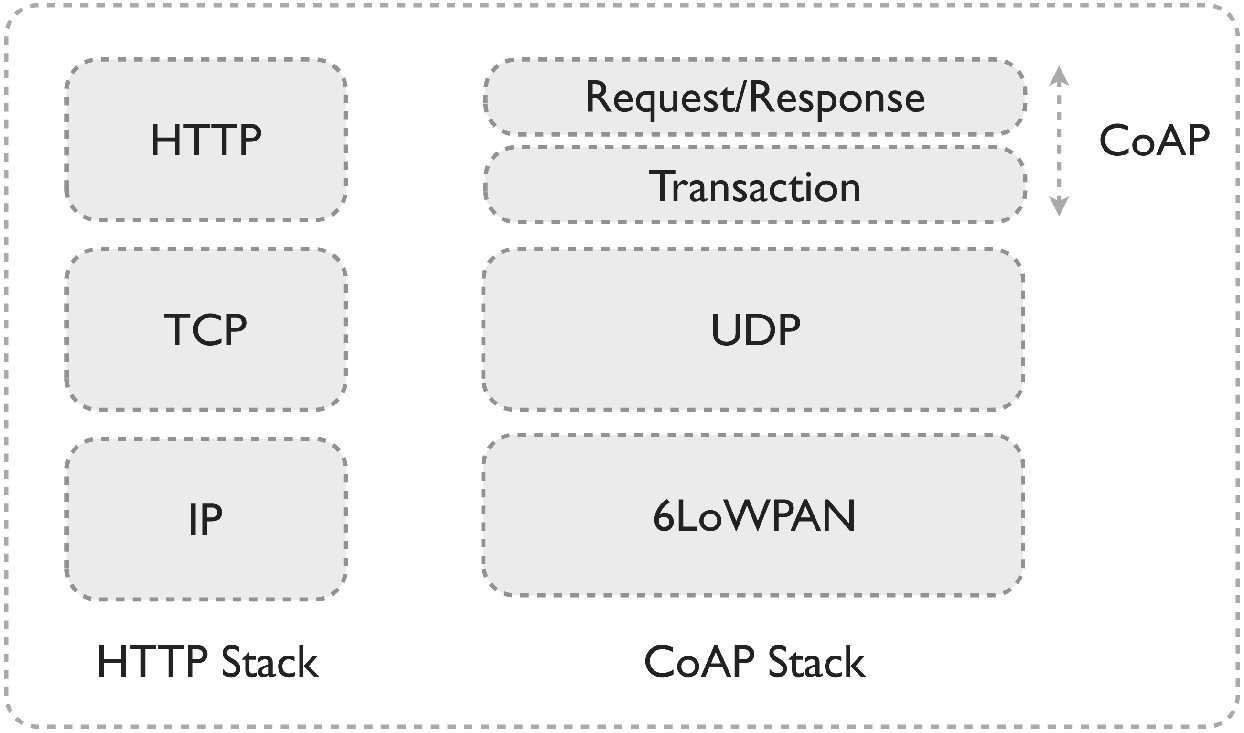
\includegraphics[width=1\textwidth]{images/http-and-coap-stack.pdf}
    \caption{HTTP and CoAP Stack Comparison}
    \label{fig:http-and-coap-stack}
  \end{center}
\end{figure}

CoAP relies on UDP. Moreover, CoAP cannot communicate with a browser directly without a gateway which translates CoAP to HTTP. The gateway can be an application. e.g. Copper\footnote{https://addons.mozilla.org/de/firefox/addon/copper-270430/}, a firefox plug-in, currently, is available for users to browse and interact with Internet of Things devices.

\section{MQTT}
Message Queuing Telemetry Transport (MQTT)\footnote{http://mqtt.org} is a machine-to-machine (M2M) / IoT connectivity protocol. There are two main specification for MQTT: MQTT v3.1 and MQTT-S (MQTT for Sensor) v1.2. We will compare MQTT V3.1 with WAMP. Since MQTT-S does not work on TCP/IP network, it is out of scope of my project.

MQTT is designed as an extremely lightweight publish/subscribe messaging transport; while MQTT-S is a publish/subscribe messaging protocol for wireless sensor networks (WSNs) and is originally designed for non-TCP/IP networks.

MQTT V3.1 and WAMP are both working on TCP/IP network. Different from WAMP, MQTT V3.1 assumes the communications channel is more likely to be unreliable.

MQTT V3.1 has a two bytes message header and a UTF8 encoded payload.
Message type, such as Pub/Sub, is defined in the header. Unlike WAMP, MQTT V3.1 does not yet support RPC. Additionally, MQTT V3.1 provides three levels of Quality of Services (QoS) control.

Level 0 is called ``At most once delivery'', when the message is delivered highly dependent to the underlying TCP/IP network. There is no any expectation that the recipient will sent back a response and the message arrives at the recipient at once or it just loses.

Level 1 is called ``At least once delivery'', when a response is expected to be sent back from the recipient, otherwise, the sender will re-send the message.

Level 2 is called ``Exactly once delivery'', when the message will be received and only received once by the recipient. More helper messages will be exchanged at this level to ensure the quality of delivery, and hence there is an increase in the network traffic \cite{MQTTV31ProtocolSpec}.

WAMP, however, does not support such QoS control. Finally, WAMP has been officially registered in the WebSocket Subprotocol Name Registry, while MQTT is not a member.

\section{Comparison}
Table \ref{table:WAMPCoAPandMQTTcomparison} is a summary of the comparison between WAMP, CoAP and MQTT.

% If you need to have linefeeds (\\) inside a cell, you must create a new
% paragraph-formatting environment inside the cell. Most common ones are 
% the minipage-environment and the \parbox command (see LaTeX documentation
% for details; or just google for ``LaTeX minipage'' and ``LaTeX parbox'').
\begin{table}
\begin{tabular}{|p{3.3cm}|>{\centering\arraybackslash}p{3cm}|>{\centering\arraybackslash}p{3cm}|>{\centering\arraybackslash}p{3.3cm}|} 
% Alignment of sells: l=left, c=center, r=right. 
% If you want wrapping lines, use p{width} exact cell widths.
% If you want vertical lines between columns, write | above between the letters
% Horizontal lines are generated with the \hline command:
\hline % The line on top of the table
\textbf{ } & \textbf{WAMP} & \textbf{CoAP} & \textbf{MQTT} \\ 
\hline 
% Place a & between the columns
% In the end of the line, use two backslashes \\ to break the line,
% then place a \hline to make a horizontal line below the row 
\textbf{Transport Layer} & TCP & UDP & TCP \\ 
\hline
\textbf{Get Resource} & over WebSockets & HTTP Requests & BSD Sockets \\
% The multicolumn command takes the following 3 arguments: 
% the number of cells to merge, the cell formatting for the new cell, and the
% contents of the cell
\hline
\textbf{Browser} & yes, HTML5 support & no, only via Firefox plugin currently & no, not directly \\
\hline
\textbf{Server} & WebSocket Server with WAMP support & CoAP Server & MQTT Server \\
\hline
\textbf{RPC} & yes & request/response model (through REST APIs) & no \\
\hline
\textbf{Pub/Sub} & yes & yes & yes \\
\hline
\textbf{Proxy Support} & through WebSockets & built-in & external proxy to translate protocol (implies delay) \\
\hline
\end{tabular} % for really simple tables, you can just use tabular
% You can place the caption either below (like here) or above the table
\caption{WAMP, CoAP and MQTT comparison}
\label{table:WAMPCoAPandMQTTcomparison}
\end{table} % table makes a floating object with a title
